%% SW design: klassebeskrivelse devkit Controllers
\newpage

\begin{figure}[htbp] \centering
{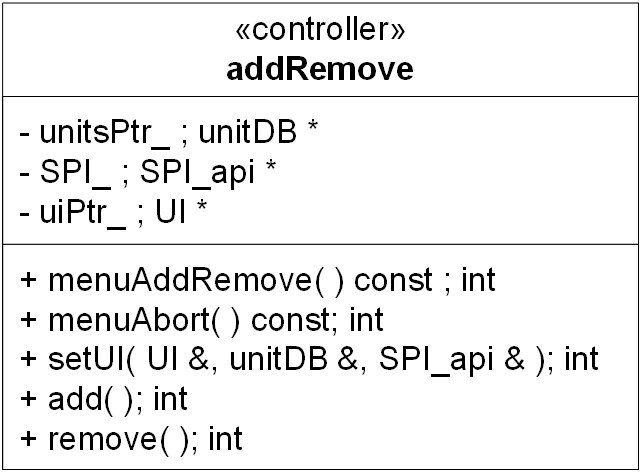
\includegraphics[scale=1.5]{filer/design/Klassediagrammer/sw_addRemove}}
\caption{klassediagram addRemove}
\label{fig:addRemove klassediagram}
\end{figure} 

{\centering
\textbf{addRemove}\par
}
\textbf{Ansvar:} at styre forløbet i UC1: Tilføj / fjern enhed. \

\verb+int menuAddRemove( ) const+ \\
\textbf{Parametre:} Modtager ingen parametre. \\
\textbf{Returværdi:} 0 ved succes ellers negativ i overenstemmelse med fejl-listen. \\
\textbf{Beskrivelse:} Modtager information fra brugeren omkring Enhed. Verificerer Enheden over SPI netværket og gemmer information i databasen.\\

\begin{figure}[htbp] \centering
{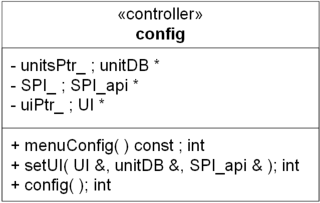
\includegraphics[scale=1.5]{filer/design/Klassediagrammer/sw_config}}
\caption{klassediagram config}
\label{fig:config klassediagram}
\end{figure} 

{\centering
\textbf{Config}\par
}
\textbf{Ansvar:} At styre forløbet i UC2: Konfig. \

\verb+int menuConfig( ) const+ \\
\textbf{Parametre:} Modtager ingen parametre. \\
\textbf{Returværdi:} 0 ved succes ellers negativ i overenstemmelse med fejl-listen. \\
\textbf{Beskrivelse:} Modtager information fra brugeren omkring Enhed og parametre. Parametrene skrives til den pågældende Enhed på SPI netværket.\\

\begin{figure}[htbp] \centering
{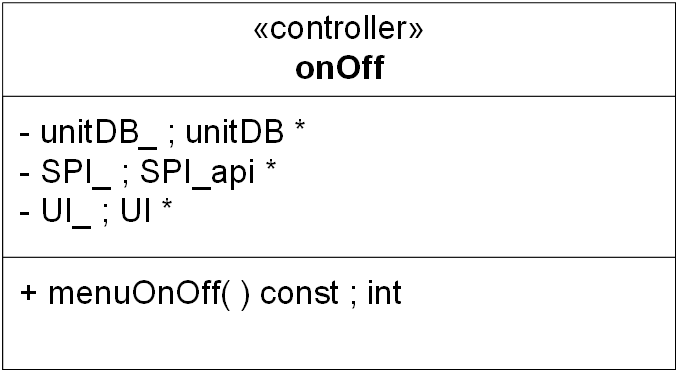
\includegraphics[scale=1.5]{filer/design/Klassediagrammer/sw_onOff}}
\caption{klassediagram onOff}
\label{fig:onOff klassediagram}
\end{figure} 

\newpage

{\centering
\textbf{onOff}\par
}
\textbf{Ansvar:} At styre forløbet i UC3: Aktiver / deaktiver. \

\verb+int menuOnOff( ) const+ \\
\textbf{Parametre:} Modtager ingen parametre. \\
\textbf{Returværdi:} 0 ved succes ellers negativ i overenstemmelse med fejl-listen. \\
\textbf{Beskrivelse:} Modtager information fra brugeren omkring hvilken Enhed som ønskes aktiveret eller deaktiveret. Enheden modtager informationen over SPI netværket.\\

\begin{figure}[htbp] \centering
{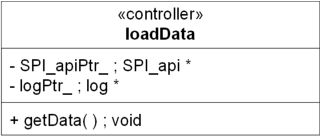
\includegraphics[scale=1.5]{filer/design/Klassediagrammer/sw_loadData}}
\caption{klassediagram loadData}
\label{fig:loadData klassediagram}
\end{figure} 

{\centering
\textbf{loadData}\par
}
\textbf{Ansvar:} At styre forløbet i UC4: Databehandling. \

\verb+void getData( )+ \\
\textbf{Parametre:} Modtager ingen parametre \\
\textbf{Returværdi:} 0 ved succes ellers negativ i overenstemmelse med fejl-listen \\
\textbf{Beskrivelse:} Kaldes af en uafhængig tråd når en timer løber ud. Skal hente log-data over SPI netværket. Kontrollerer om der er nogle sensor-læsninger i mellem dataen og gemme denne i \verb+log+-objektet. Fejl gemmes ikke i \verb+log+.\\

\begin{figure}[htbp] \centering
{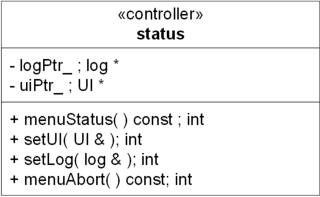
\includegraphics[scale=1.5]{filer/design/Klassediagrammer/sw_status}}
\caption{klassediagram status}
\label{fig:status klassediagram}
\end{figure} 

\newpage

{\centering
\textbf{status}\par
}
\textbf{Ansvar:} at styre forløbet i UC5: Tjek status. \

\verb+int menuStatus( ) const+ \\
\textbf{Parametre:} Modtager ingen parametre. \\
\textbf{Returværdi:} 0 ved succes ellers negativ i overenstemmelse med fejl-listen. \\
\textbf{Beskrivelse:} Henter den seneste log i hukommelsen og viser brugeren den, for den ønskede Enhed.\\

\begin{figure}[htbp] \centering
{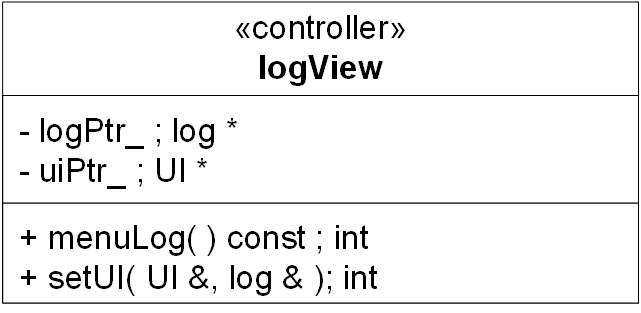
\includegraphics[scale=1.5]{filer/design/Klassediagrammer/sw_logView}}
\caption{klassediagram logView}
\label{fig:logView klassediagram}
\end{figure}

{\centering
\textbf{logView}\par
}
\textbf{Ansvar:} at styre forløbet i UC6: Udskriv log. \

\verb+int menuLog( ) const+ \\
\textbf{Parametre:} Modtager ingen parametre. \\
\textbf{Returværdi:} 0 ved succes ellers negativ i overenstemmelse med fejl-listen. \\
\textbf{Beskrivelse:} Henter hele loggen i hukommelsen og viser brugeren den, for den ønskede Enhed.\\

